\chapter{Разработка модели обработки}
\label{sec:research:development_model}

Начать разработку следует с модели предствления динамических данных. Модель должна соответсвовать следующим критериям:

\begin{itemize}
  \item иметь возможность предоставить данные;
  \item сообщить, когда они изменятся.
\end{itemize}

В \dotnet{} уже существует интейфейсы, которые предоставляют данную функциональность:

\begin{itemize}
  \item \lstinline[style=csharpinlinestyle]!IReadOnlyCollection! --- предоставляет доступ для чтения набора данных~\cite{ireadonlycollection};
  \item \lstinline[style=csharpinlinestyle]!IReadOnlyList! --- предоставляет доступ для чтения набора данных,
  наследуется от \lstinline[style=csharpinlinestyle]!IReadOnlyCollection! и предоставляет доступ по индексу~\cite{ireadonlylist};
  \item \lstinline[style=csharpinlinestyle]!INotifyCollectionChanged! --- содержит событие, подписавшись на которое, можно следить за изменением набора данных~\cite{inotifycollectionchanged}.
\end{itemize}

В моей модели я использую только первых два интерфейса и два интерфейса, которые заменяют \lstinline[style=csharpinlinestyle]!INotifyCollectionChanged!.
Я использую свой интерфейс, потому что \lstinline[style=csharpinlinestyle]!INotifyCollectionChanged! имеет ряд недостатков:

\begin{itemize}
  \item не может сообщить о изменении коллекции без индексов;
  \item реализовано через стандартную модель Event --- это вызвало бы нагромождение однообразного кода, при реализации операций обработки данных;
  \item со стандартными Event нельзя строить LINQ выражения для работы с событиями по принципам функционального программирования.
\end{itemize}

Далее я опишу получившуюся модель для динамических наборов данных.

\section{Модели событий обновления наборов данных}
\label{sub:research:event_model}

Для замены \lstinline[style=csharpinlinestyle]!INotifyCollectionChanged! в моей модели существуют два интефейса:
\lstinline[style=csharpinlinestyle]!INotifyCollectionChanged<out T>! и \lstinline[style=csharpinlinestyle]!INotifyListChanged<out T>!.
Как можно заметить, первый служит для обычных коллекций, а второй для списков.

\begin{figure}[ht]
\centering
  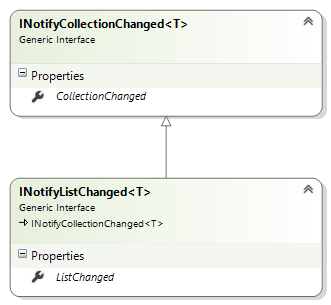
\includegraphics[scale=0.85]{event_generators.png}
  \caption{ Интерфейсы генераторов событий для наборов данных }
  \label{fig:event_generators}
\end{figure}

Рассмотрим их подробнее. Свойство генератора событий обновления коллекции \lstinline[style=csharpinlinestyle]!CollectionChanged! имеет тип \lstinline[style=csharpinlinestyle]!IObservable!.
Если подписаться на это событие, то получатель будет иметь в своем распоряжении объекты типа \lstinline[style=csharpinlinestyle]!IUpdateCollectionQuery!,
который является алегбраическим типом данных и представляет тип-сумму~\cite{algebraic_data_type}.
\lstinline[style=csharpinlinestyle]!IUpdateCollectionQuery! --- является объектом запроса на обновление коллекции.
Он является суммой данных типов:

\begin{itemize}
  \item \lstinline[style=csharpinlinestyle]!ICollectionOnInsertArgs<T>! --- запрос на вставку одного элемента типа T в коллекцию. Содержит ссылку на добавляемый объект типа T;
  \item \lstinline[style=csharpinlinestyle]!ICollectionOnRemoveArgs<T>! --- запрос на удаление одного элемента типа T из коллекции. Содержит ссылку на удаляемый объект типа T;
  \item \lstinline[style=csharpinlinestyle]!ICollectionOnReplaceArgs<T>! --- запрос на замену одного элемента типа T, другим элементов типа T в коллекции. Содержит ссылки на старый и новый объекты типа T;
  \item \lstinline[style=csharpinlinestyle]!ICollectionOnResetArgs<T>! --- замена всего содержимого коллекции. Содержит список исходных объектов коллекции и новый список объектов коллекции;
  \item \lstinline[style=csharpinlinestyle]!ICollectionOnEmptyArgs<T>! --- пустой запрос. Ничего не содержит.
\end{itemize}

\lstinline[style=csharpinlinestyle]!ListChanged! имеет тип \lstinline[style=csharpinlinestyle]!IObservable<IUpdateListQuery>!.
Если подписаться на это событие, то получатель будет иметь в своем распоряжении объекты типа \lstinline[style=csharpinlinestyle]!IUpdateListQuery!,
который является алегбраическим типом данных и представляет тип-сумму~\cite{algebraic_data_type}.
\lstinline[style=csharpinlinestyle]!IUpdateListQuery! --- является объектом запроса на обновление списка.
Он является суммой данных типов:

\begin{itemize}
  \item \lstinline[style=csharpinlinestyle]!IListOnInsertArgs<T>! --- запрос на вставку одного элемента типа T в список. Содержит ссылку на добавляемый объект типа T и позицию для вставки;
  \item \lstinline[style=csharpinlinestyle]!IListOnRemoveArgs<T>! --- запрос на удаление одного элемента типа T из списка. Содержит ссылку на удаляемый объект типа T и позицию удаления;
  \item \lstinline[style=csharpinlinestyle]!IListOnReplaceArgs<T>! --- запрос на замену одного элемента типа T, другим элементов типа T в списке.
  Содержит ссылки на старый и новый объекты типа T и позицию исходного элемента;
  \item \lstinline[style=csharpinlinestyle]!IListOnMoveArgs<T>! --- запрос на перемещение одного элемента типа T. Содержит ссылку объект типа T, исходную и новую позиции;
  \item \lstinline[style=csharpinlinestyle]!IListOnResetArgs<T>! --- замена всего содержимого списка. Содержит список исходных объектов списка и новый список объектов списка;
  \item \lstinline[style=csharpinlinestyle]!IListOnEmptyArgs<T>! --- пустой запрос. Ничего не содержит.
\end{itemize}

На рисунке~\ref{fig:queries} видно как соотносятся между собой запросы. Запросы для списков подходят в качестве запросов для коллекций.
Данная модель учитывает то, что каждый список по сути является коллекцией и наследует её признаки.

\begin{figure}[ht]
\centering
  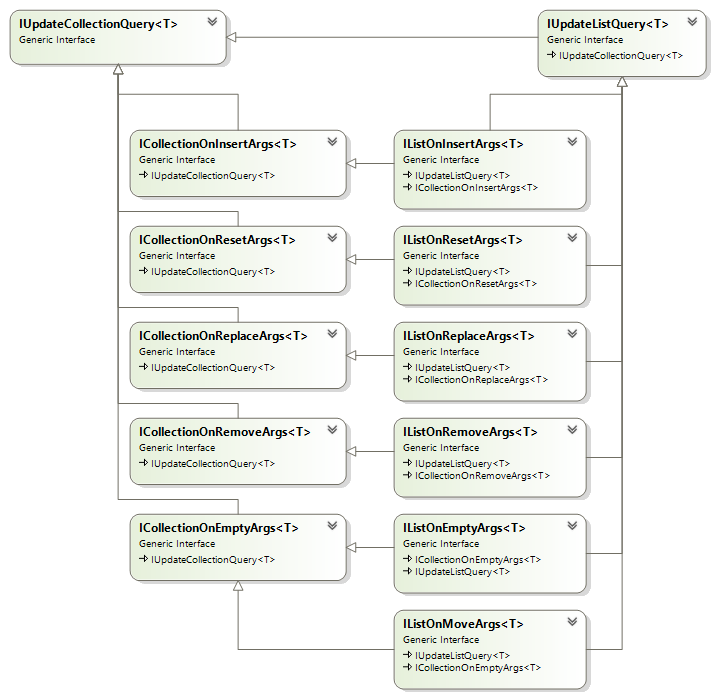
\includegraphics[scale=0.85]{queries.png}
  \caption{ Схема наследования запросов }
  \label{fig:queries}
\end{figure}

Интерфейсы, которые объединяют генераторы событий и хранилища данных именуются \lstinline[style=csharpinlinestyle]!IObservableReadOnlyCollection! для коллекций, а также \lstinline[style=csharpinlinestyle]!IObservableReadOnlyList! для списков.
Лист наследуется коллекции. В данной модели разработаны и реалицации этих коллекций и списков, которые можно изменять. Эти реализации и будут отправной точкой событий в данной системе.
В модели они выражены в интерфейсах:

\begin{itemize}
  \item \lstinline[style=csharpinlinestyle]!IObservableCollection<T>! --- наследует шаблонный интерфейс коллекции с разрешением только на чтение \lstinline[style=csharpinlinestyle]!IObservableReadOnlyCollection<T>! и редактируемой --- \lstinline[style=csharpinlinestyle]!ICollection<T>!.
  Расширен методами Replace и Reset. Первый позволяет одиним событием заменять элемент в коллекции, а второй позволяет сбрасывать содержимое коллекции за одно событие;
  \item \lstinline[style=csharpinlinestyle]!IObservableList<T>! --- наследует шаблонный интерфейс списка с разрешением только на чтение \lstinline[style=csharpinlinestyle]!IObservableReadOnlyList<T>!, с возможностью редактирования --- \lstinline[style=csharpinlinestyle]!IList<T>! и \lstinline[style=csharpinlinestyle]!IObservableCollection<T>!.
  Расширен методами Replace, Reset и Move. Первые два, действуют аналогично методам из интерфейса коллекции, а метод Move позволяет изменять положение объекта за одно событие.
\end{itemize}

\lstinline[style=csharpinlinestyle]!IObservableCollection<T>! --- наследует интерфейс \lstinline[style=csharpinlinestyle]!ITransactional!, который позволяет выполнять несколько операций подряд, не генерируя при этом событий.
События сгенерируются только по завершению транзакции.

\begin{figure}[ht]
\centering
  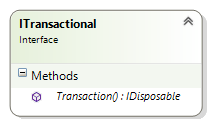
\includegraphics[scale=0.85]{transaction.png}
  \caption{ Интерфейс для создания транзакций }
  \label{fig:transaction}
\end{figure}

\begin{lstlisting}[style=csharpinlinestyle, caption={Использование транзакции}, label=lst:practice:development_model:transaction_example]
  IObservableCollection<int> collection = new ObservableCollection<int>();

  using(collection.Transaction())
  {
    collection.Add(5);
    collection.Add(2);
    collection.Add(1);
  }
\end{lstlisting}

В листинге~\ref{lst:practice:development_model:transaction_example} транзакция создается и завершается в блоке using.
Все операции что находятся внутри блока, сгенерируют события, когда у объекта транзакции выховется метод \lstinline[style=csharpinlinestyle]!Dispose!.

\section{Модели операций над наборами данных}
\label{sub:research:operational_model}

Операция --- в контексте данной модели, это преобразование набора данных. Такое преобразование можно описать так: один набор данных по заданному правилу преоразуется в другой набор данных.
Я выделил пять видов преобразований:

\begin{itemize}
  \item коллекция объектов типа TIn преобразуется в коллекцию объектов типа TOut;
  \item коллекция объектов типа TIn преобразуется в упорядоченный список объектов типа TOut;
  \item список объектов типа TIn преобразуется в список объектов TOut;
  \item вычисление функции на основе коллекции объектов типа T;
  \item вычисление функции на основе списка объектов типа T.
\end{itemize}

\begin{figure}[ht]
\centering
  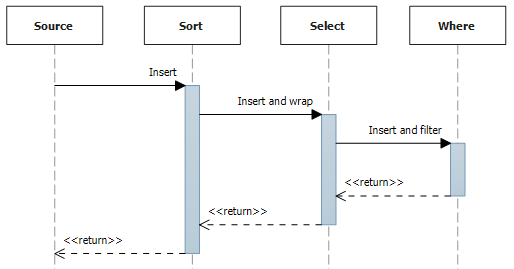
\includegraphics[scale=0.85]{operation_diagram.png}
  \caption{ Диаграмма взаимодействия наборов данных }
  \label{fig:operation_diagram}
\end{figure}

\begin{lstlisting}[style=csharpinlinestyle, caption={Пример применения операций}, label=lst:practice:development_model:operations_example]
  var resultCollection = source.SortRc(...).SelectRl(...).WhereRl(...);
  source.Add(number);
\end{lstlisting}

Операция описывается декларативно, и создает связь между исходным объектом и получившимся. Объект, который является реализацией конкретной операции, подписывыется на изменение исходного набора и, в соответсвии
со своим назначением, изменяет зависимый набор. На рисунке~\ref{fig:operation_diagram} описан процесс взаимодействия источника(Source) и наборов, которые получились после применения операций.
Код, который соответсвует рисунку~\ref{fig:operation_diagram}, столь же простой. Его можно увидеть в листинге~\ref{lst:practice:development_model:operations_example}.

Для преобразорваний из одного типа набора в другой, было разработано три базовых класса операций:

\begin{itemize}
  \item \lstinline[style=csharpinlinestyle]!CollectionToCollectionOperationBase<TIn, TOut>! --- коллекция объектов типа TIn преобразуется в коллекцию объектов типа TOut;
  \item \lstinline[style=csharpinlinestyle]!CollectionToListOperationBase<TIn, TOut>! --- коллекция объектов типа TIn преобразуется в упорядоченный список объектов типа TOut;
  \item \lstinline[style=csharpinlinestyle]!ListToListOperationBase<TIn, TOut>! --- список объектов типа TIn преобразуется в список объектов TOut.
\end{itemize}

Для функций были разработаны следующий базовые классы:

\begin{itemize}
  \item \lstinline[style=csharpinlinestyle]!CollectionFunctionBase<T>! --- вычисление функции на основе коллекции объектов типа T;
  \item \lstinline[style=csharpinlinestyle]!ListFunctionBase<T>! --- вычисление функции на основе списка объектов типа T.
\end{itemize}

Рассмотрим каждый из разработанных базовых реализаций, выделив ключевые детали.

\begin{figure}[ht]
\centering
  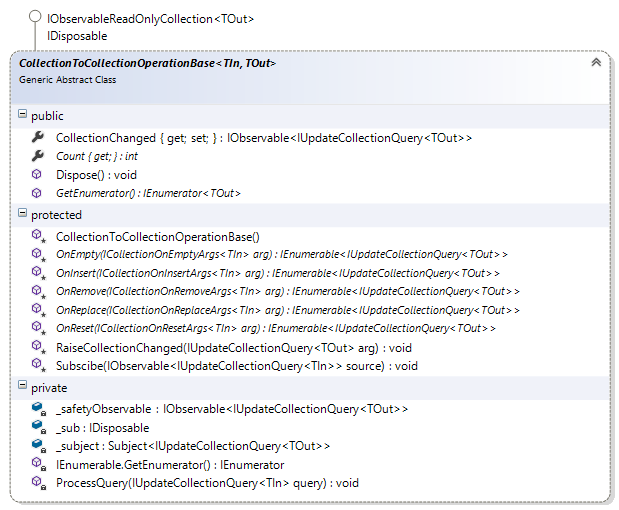
\includegraphics[scale=0.85]{collection_to_collection_operation_base.png}
  \caption{ Операция преобразования коллекции в коллекцию }
  \label{fig:collection_to_collection_operation_base}
\end{figure}

\lstinline[style=csharpinlinestyle]!CollectionToCollectionOperationBase<TIn, TOut>! --- наследуется от  интерфейса \lstinline[style=csharpinlinestyle]!IObservableReadOnlyCollection<TOut>!
и предназеначен для работы с генераторами событий \lstinline[style=csharpinlinestyle]!IObservable<IUpdateCollectionQuery<TIn>!(см. рисунок~\ref{fig:collection_to_collection_operation_base}).
Позволяет реализовать операции трансформации(Select), фильтрации(Where) и т. д. Например: преобразование увеличения целых чисел в 2 раза или фильтрация записей студентов по группе.
Результат будет обновлятся вместе исходной коллекцией. Класс решает задачи:

\begin{itemize}
  \item подписывается на источник событий с помощью Weak reference(слабой ссылки)\cite{weak_reference};
  \item создает пустые реализации для всех существующих типов запросов; если запрос не был обработан, возникнет ошибка на этапе компиляции;
  \item реализует интерфейс \lstinline[style=csharpinlinestyle]!IObservableReadOnlyCollection<TOut>!;
  \item генерирует события для \lstinline[style=csharpinlinestyle]!IObservableReadOnlyCollection<TOut>!.
\end{itemize}

\begin{figure}[ht]
\centering
  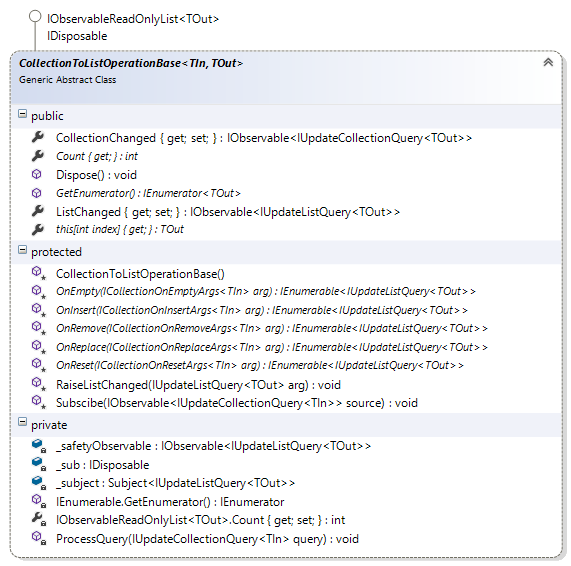
\includegraphics[scale=0.85]{collection_to_list_operation_base.png}
  \caption{ Операция преобразования коллекции в список }
  \label{fig:collection_to_list_operation_base}
\end{figure}

\lstinline[style=csharpinlinestyle]!CollectionToListOperationBase<TIn, TOut>! --- наследуется от базового интерфейса \lstinline[style=csharpinlinestyle]!IObservableReadOnlyList<TOut>!
и предназеначен для работы с генераторами событий \lstinline[style=csharpinlinestyle]!IObservable<IUpdateCollectionQuery<TIn>!(см. рисунок~\ref{fig:collection_to_list_operation_base}).
Позволяет реализовать операции по упорядочиванию элементов(Sort). Например: требуется сортировать заказы учитывая приоритет, который может измениться.
Операция будет учитывать не только добавление и удаление элементов из коллекции, а еще и отслеживать изменения ключа сортировки.
Класс решает задачи:

\begin{itemize}
  \item подписывается на источник событий при помощи Weak reference;
  \item создает пустые реализации для всех существующих типов запросов; если запрос не был обработан, возникнет ошибка на этапе компиляции;
  \item реализует интерфейс \lstinline[style=csharpinlinestyle]!IObservableReadOnlyList<TOut>!;
  \item генерирует события для \lstinline[style=csharpinlinestyle]!IObservableReadOnlyList<TOut>!.
\end{itemize}

\begin{figure}[ht]
\centering
  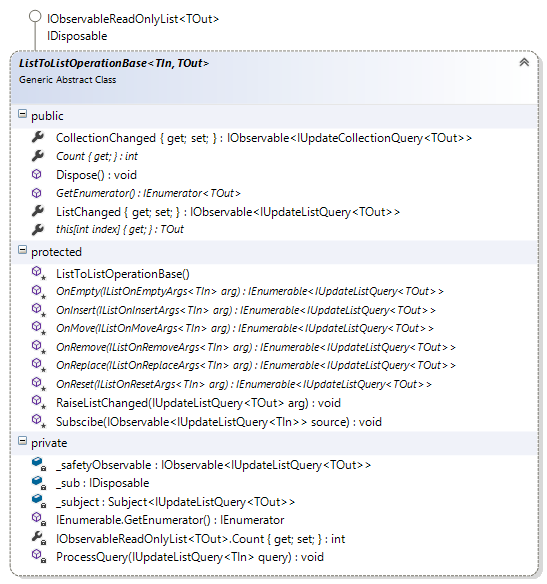
\includegraphics[scale=0.85]{list_to_list_operation_base.png}
  \caption{ Операция преобразования списка в список }
  \label{fig:list_to_list_operation_base}
\end{figure}

\lstinline[style=csharpinlinestyle]!ListToListOperationBase<TIn, TOut>! --- наследуется от базового интерфейса \lstinline[style=csharpinlinestyle]!IObservableReadOnlyList<TOut>!
и предназеначен для работы с генераторами событий \lstinline[style=csharpinlinestyle]!IObservable<IUpdateListQuery<TIn>!(см. рисунок~\ref{fig:list_to_list_operation_base}).
Позволяет реализовать операции трансформации(Select), фильтрации(Where) и т. д. Может использоваться для переупорядочивания элементов(Sort, Take, Skip).
Довольно распространённая задача реверсивного объода списка. Можно описать операцию Reverse, которая будет содержать объекты с обратной сортировкой и генерировать соответсвующие события.
Класс решает задачи:

\begin{itemize}
  \item подписывается на источник событий при помощи Weak reference;
  \item создает пустые реализации для всех существующих типов запросов; если запрос не был обработан, возникнет ошибка на этапе компиляции;
  \item реализует интерфейс \lstinline[style=csharpinlinestyle]!IObservableReadOnlyList<TOut>!;
  \item генерирует события для \lstinline[style=csharpinlinestyle]!IObservableReadOnlyList<TOut>!.
\end{itemize}

\begin{figure}[ht]
\centering
  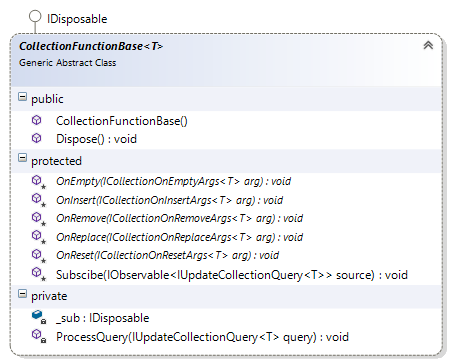
\includegraphics[scale=0.85]{collection_function_base.png}
  \caption{ Функция для коллекции }
  \label{fig:collection_function_base}
\end{figure}

\lstinline[style=csharpinlinestyle]!CollectionFunctionBase<T>! --- предназеначен для работы с генераторами событий
\lstinline[style=csharpinlinestyle]!IObservable<IUpdateCollectionQuery<TIn>!(см. рисунок~\ref{fig:collection_function_base}).
Позволяет реализовать функции подсчета(Count), поиска минимума/максимума(Min/Max) и т. д.
Можно реализовать функцию, которая будет возвращать объект с изменяющимся числом в соответствии с количеством контактов в адресной книге.
При добавлении контактов, число автоматически будет увеличиваться, при замене контакта число останется неизменным.
Класс решает задачи:

\begin{itemize}
  \item подписывается на источник событий при помощи Weak reference;
  \item создает пустые реализации для всех существующих типов запросов; если запрос не был обработан, возникнет ошибка на этапе компиляции.
\end{itemize}

\begin{figure}[ht]
\centering
  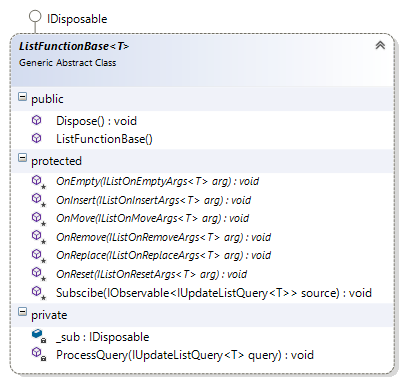
\includegraphics[scale=0.85]{list_function_base.png}
  \caption{ Функция для списка }
  \label{fig:list_function_base}
\end{figure}

\lstinline[style=csharpinlinestyle]!ListFunctionBase<T>! --- предназеначен для работы с генераторами событий
\lstinline[style=csharpinlinestyle]!IObservable<IUpdateListQuery<TIn>!(см. рисунок~\ref{fig:list_function_base}).
Позволяет реализовать функции подсчета(Count), поиска минимума/максимума(Min/Max) и т. д. Например: посчитать количесво чётных числел на нечётных местах или какая-либо другая функция,
зависящая от индексов. Можно реализовать функцию, которая будет учитывать индексы при вычислении.
Класс решает задачи:

\begin{itemize}
  \item подписывается на источник событий при помощи Weak reference;
  \item создает пустые реализации для всех существующих типов запросов; если запрос не был обработан, возникнет ошибка на этапе компиляции.
\end{itemize}

Создание данных абстрактных типов позволяет сокрыть детали реализации событийной модели. Это позволит оградить разработчика от реализации собственных способов обработки
событий для наборов данных. Потребуется только переопределить конкретные базовых классов, что ограничивает область изменений.
Изменив, что-либо в реализации одной операции --- это никак не повлияет на остальные. Названия методов и свойств подобраны для повышения информативности реализуемых методов.
Каждый метод выполняет конкретную задачу, поставленую запросом на обновления из события. Данное решение позволяет легко писать тесты для конкретных методов и оптимизировать для
конкретных случаев. Текущие базовые классы ограничивают область видимости некоторых объектов для разработчика. Например: они сами создают объект подписки и сами его отпускают, когда
ссылку на результат операции или функции никто не хранит. Но самая важная делать, что дают объекты данной модели --- это возможность работы с сущностями реального мира,
а не низкоуровневыми деталями реализации, потому что типы в модели сформированы исключительно в терминах функционального программирования, скрывая реализацию, основанную на реактивной парадигме.
Данные классы позволяют реализовать свои операции, и если потребуется, создать дополнительные абстрактные типы.
